
\section{Design}

\vspace{20mm}



\begin{abstract}

    This chapter is dedicated to representing the design of the system through a variety of different UML diagrams.


\end{abstract}

\vspace{20mm}

\large{\textbf{Outline}}

\begin{center}
    \begin{itemize}
        \item Architecture Diagram
        \item Entity Relationship Diagram
        \item Data Dictionary Diagram
        \item Data Flow Diagram
        \item Activity Diagram
        \item Sequence Diagram
        \item Collaboration Diagram
        \item State Transition Diagram
        \item Component Diagram
        \item Deployment Diagram
    \end{itemize}
\end{center}
\pagebreak


% Architecture Diagram
\subsection{Architecture Diagram}
\begin{figure}[H]
    \centering
    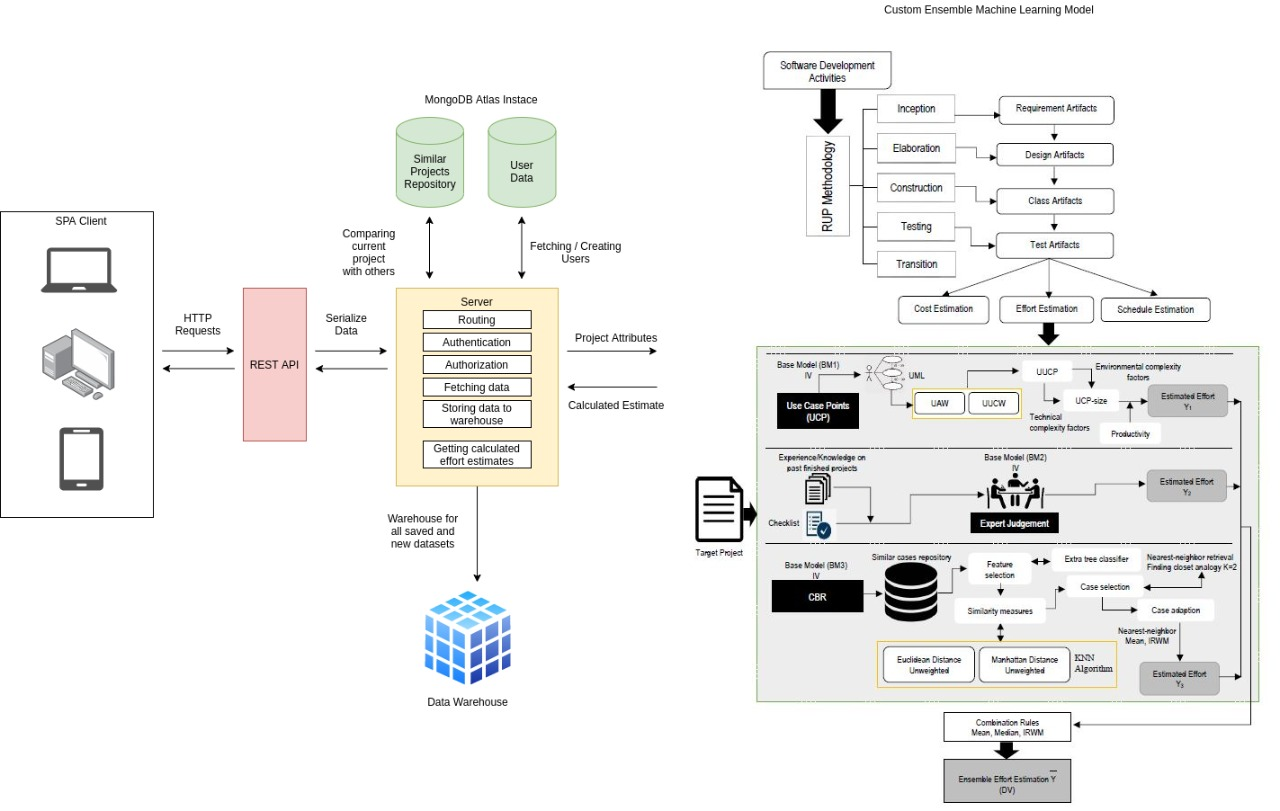
\includegraphics[scale=0.4]{./diagrams/architecture-diagram.jpeg}
    \caption{Architecture Diagram}
    \label{fig:arch-diag}

\end{figure}


% Entity Relationship Diagram
\subsection{Entity Relationship Diagram}
\begin{figure}[H]
    \centering
    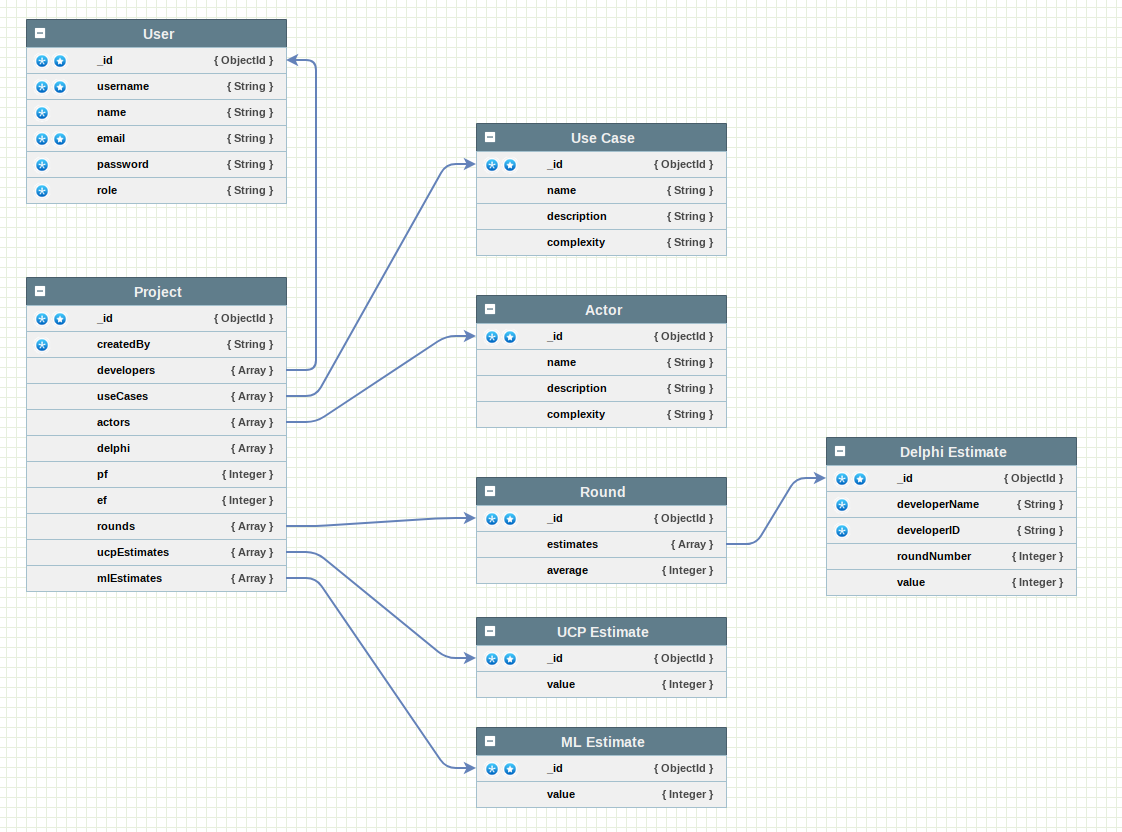
\includegraphics[scale=0.4]{./diagrams/ERD.png}
    \caption{Entity Relationship Diagram}
    \label{fig:er-diag}

\end{figure}


% Data Dictionary Diagram

\subsection{Data Dictionary Diagram}


\begin{figure}[H]
    \centering
    \caption{Data Dictionary Diagram 1}
    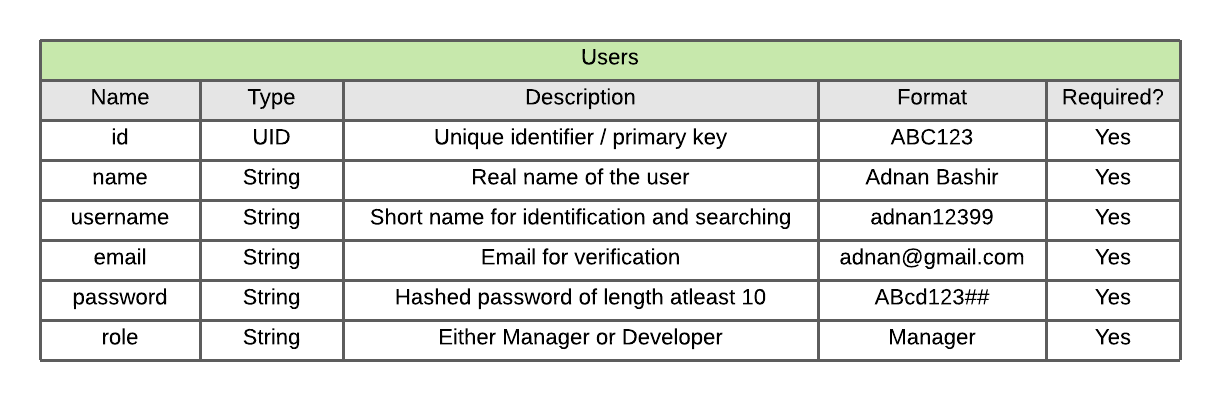
\includegraphics[scale=0.7]{./diagrams/data-dictionary/dd-1.png}
    \label{fig:dd-diag-1}

\end{figure}


\begin{figure}[H]
    \centering
    \caption{Data Dictionary Diagram 2}
    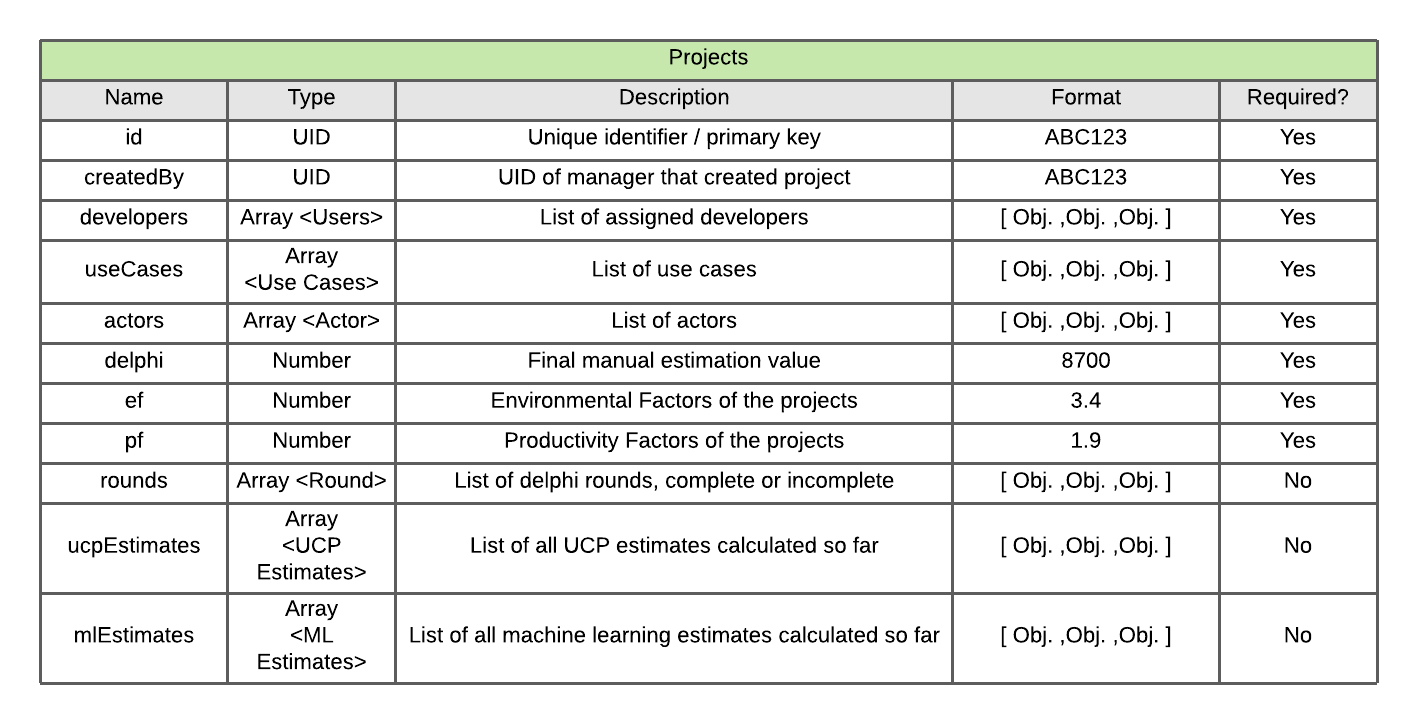
\includegraphics[scale=0.7]{./diagrams/data-dictionary/dd-2.png}
    \label{fig:dd-diag-2}
\end{figure}


\begin{figure}[H]
    \centering
    \caption{Data Dictionary Diagram 3}
    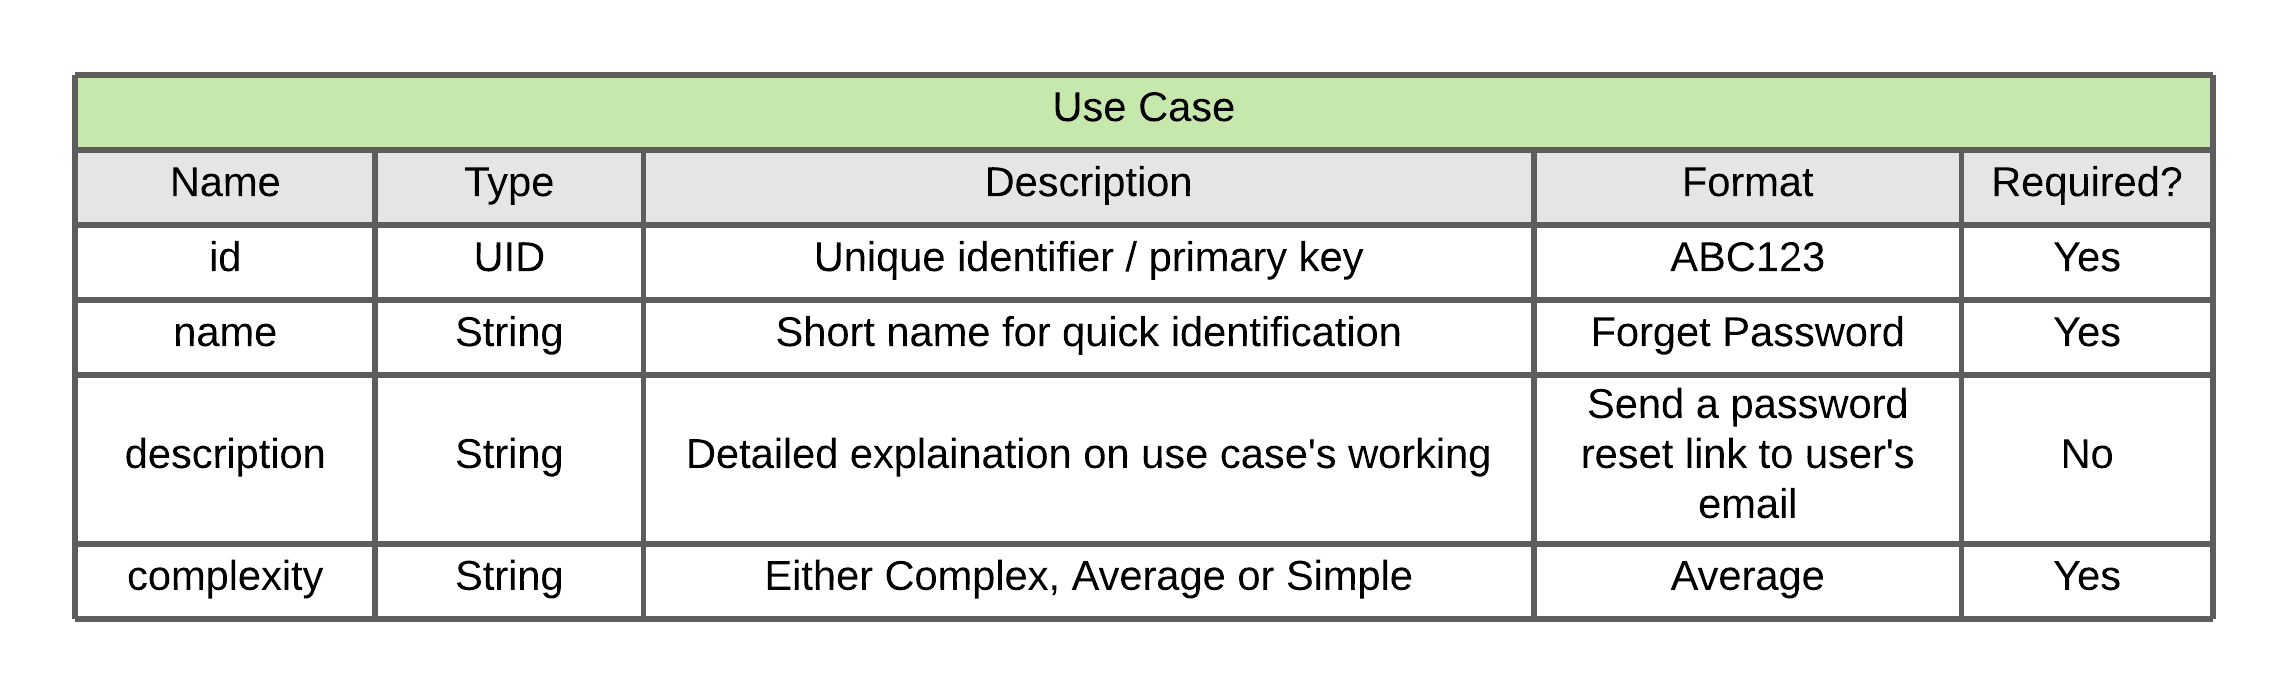
\includegraphics[scale=0.7]{./diagrams/data-dictionary/dd-3.png}
    \label{fig:dd-diag-3}

\end{figure}


\begin{figure}[H]
    \centering
    \caption{Data Dictionary Diagram 4}
    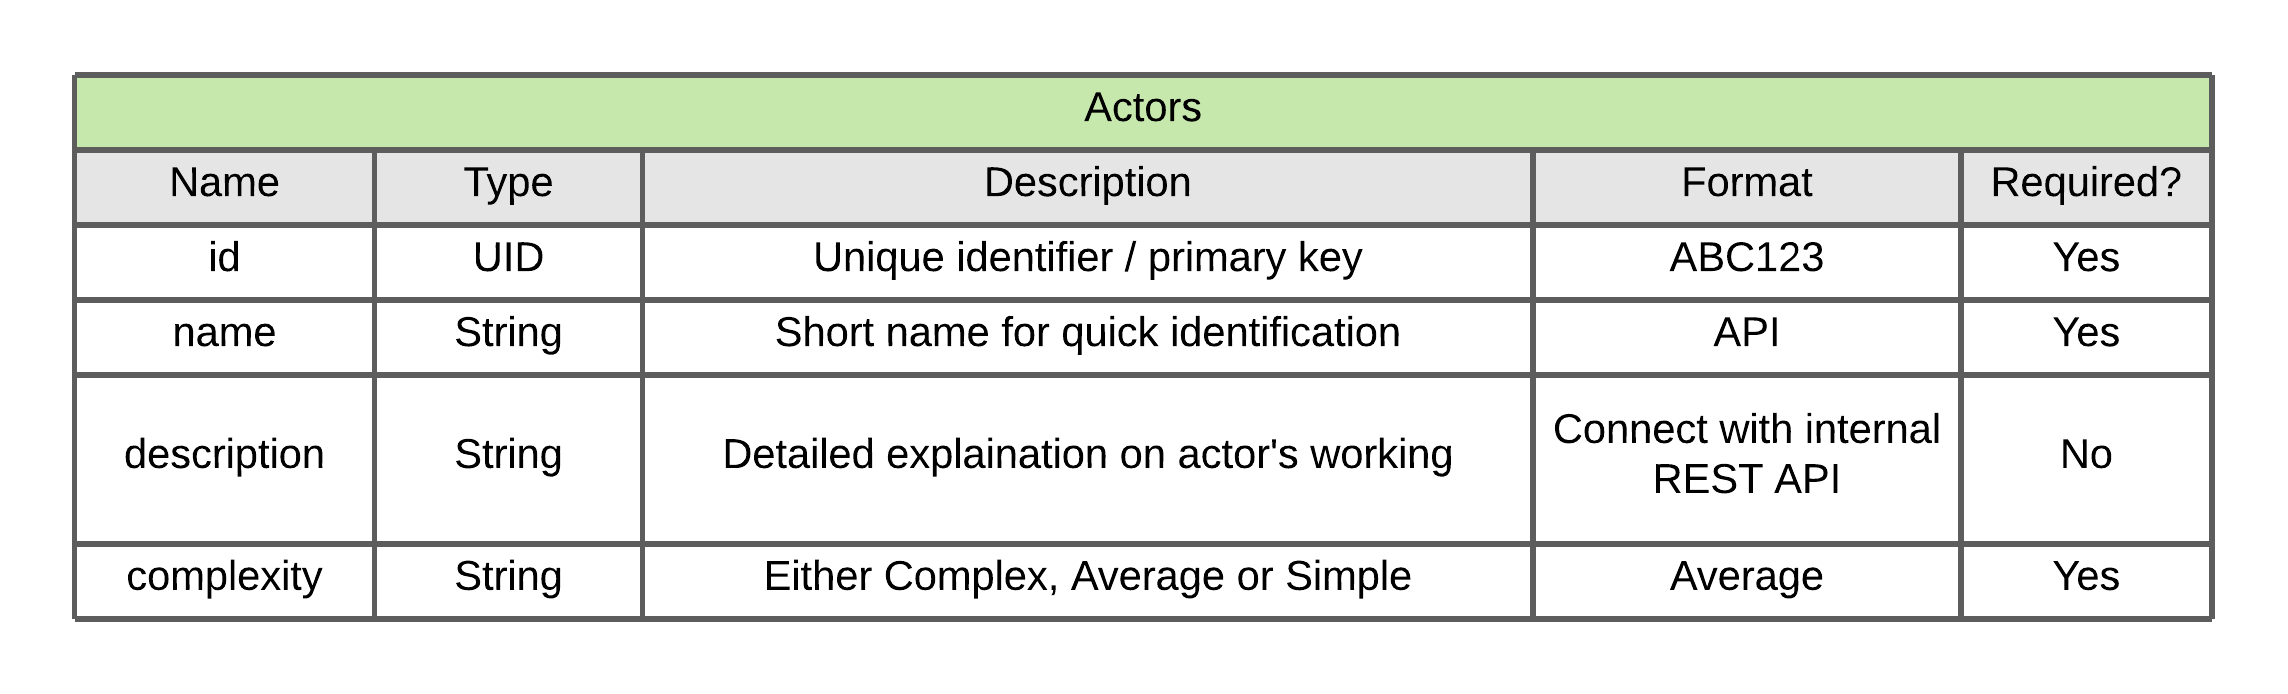
\includegraphics[scale=0.7]{./diagrams/data-dictionary/dd-4.png}
    \label{fig:dd-diag-4}

\end{figure}


\begin{figure}[H]
    \centering
    \caption{Data Dictionary Diagram 5}
    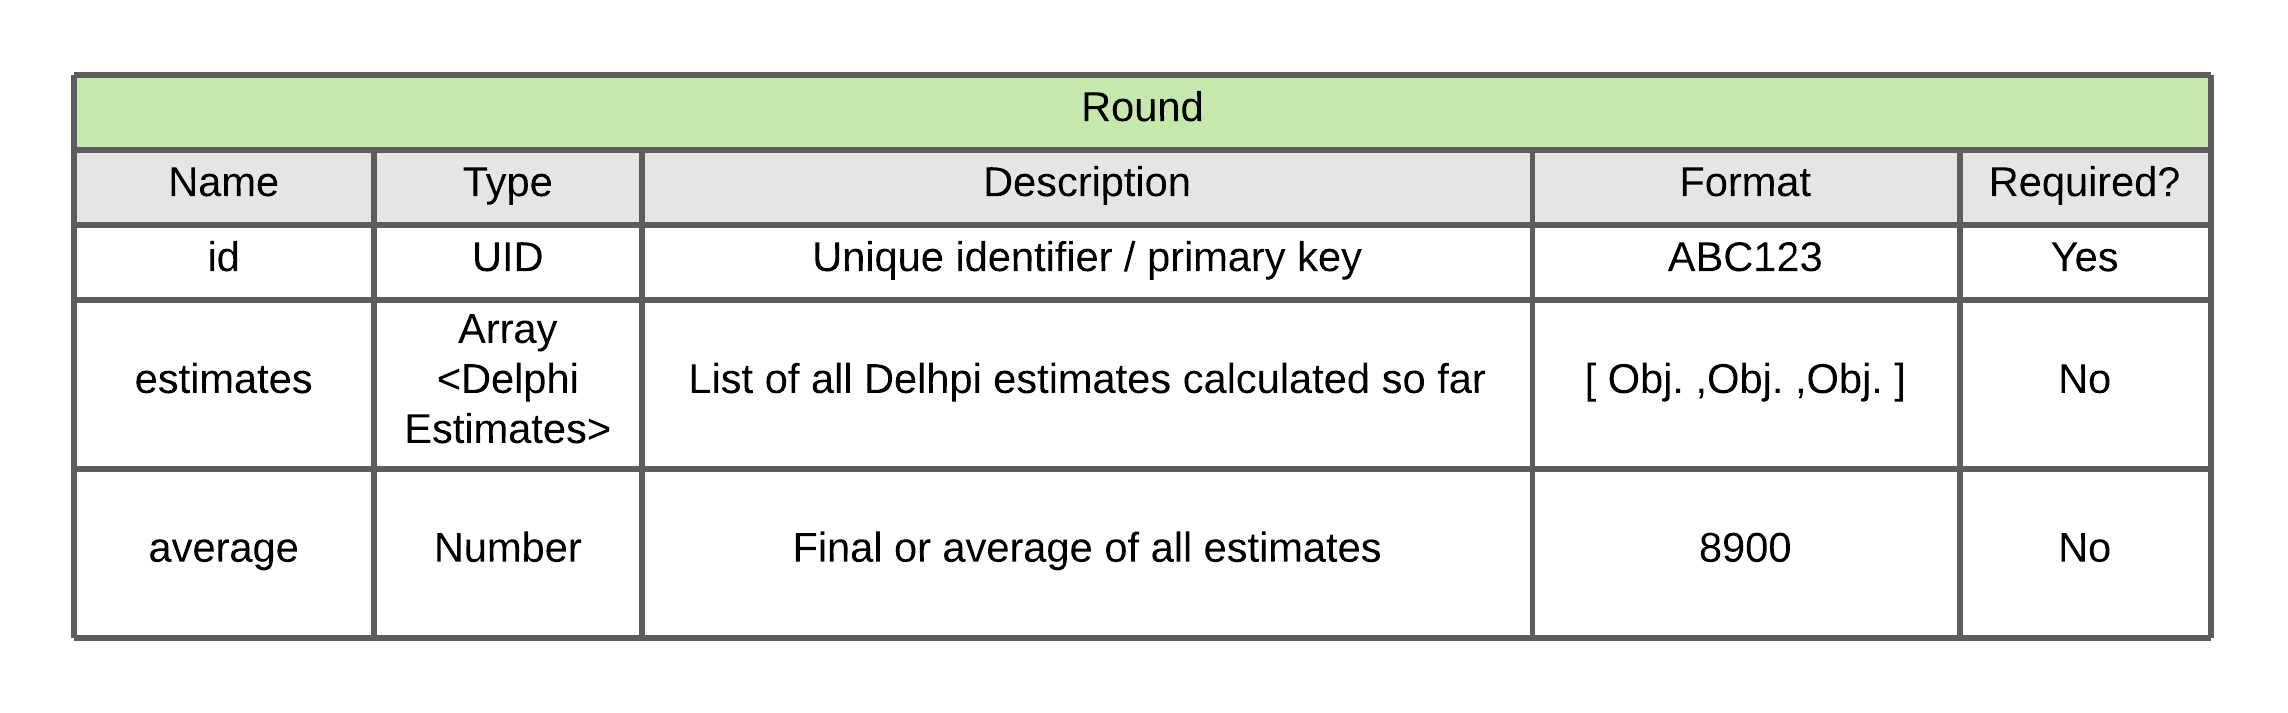
\includegraphics[scale=0.7]{./diagrams/data-dictionary/dd-5.png}
    \label{fig:dd-diag-5}

\end{figure}



\begin{figure}[H]
    \centering
    \caption{Data Dictionary Diagram 6}
    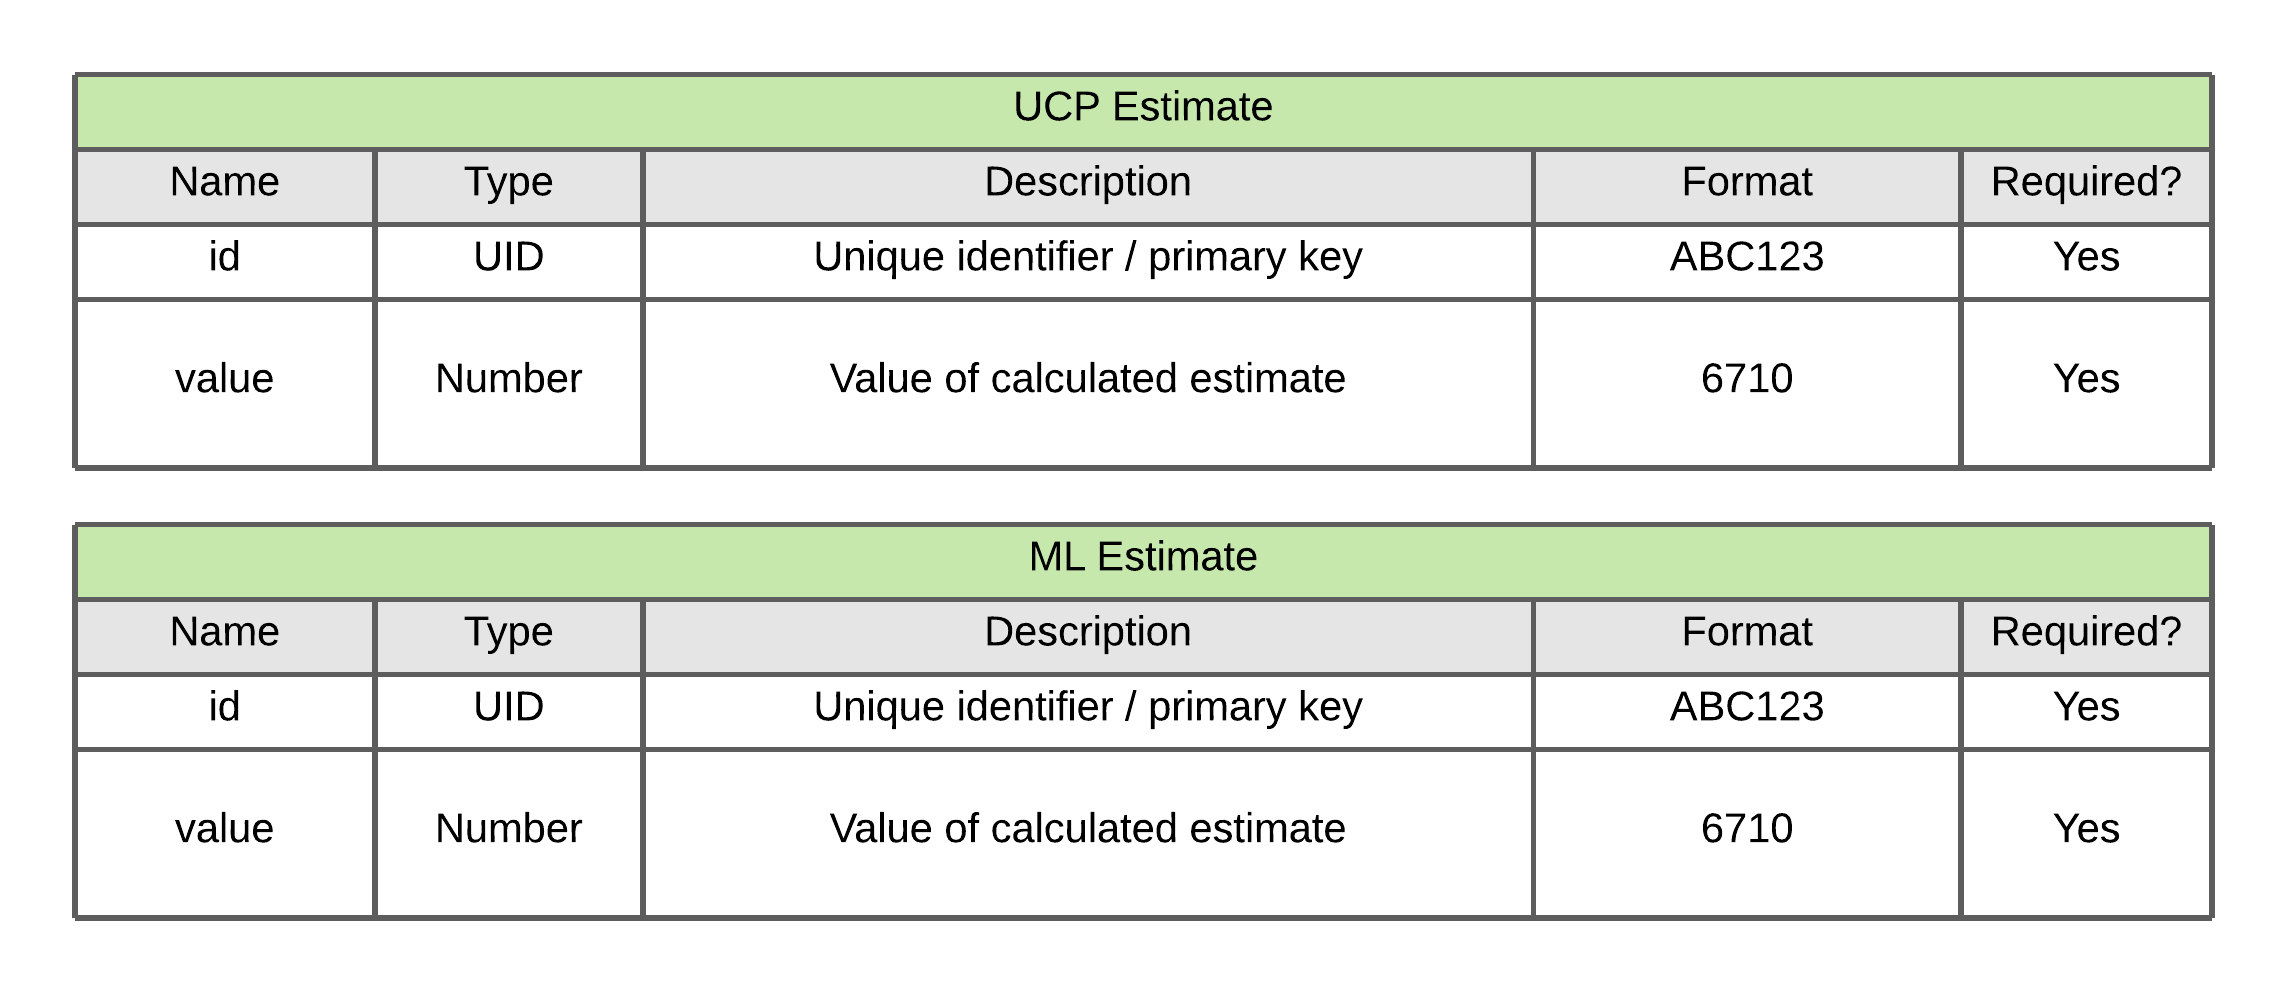
\includegraphics[scale=0.7]{./diagrams/data-dictionary/dd-6.png}
    \label{fig:dd-diag-6}
\end{figure}

% Data Flow Diagram
% Data Flow Diagram
\subsection{Data Flow Diagram}

\subsubsection{Level 1}

\begin{figure}[H]
    \centering
    \caption{Data Flow Diagram 1}
    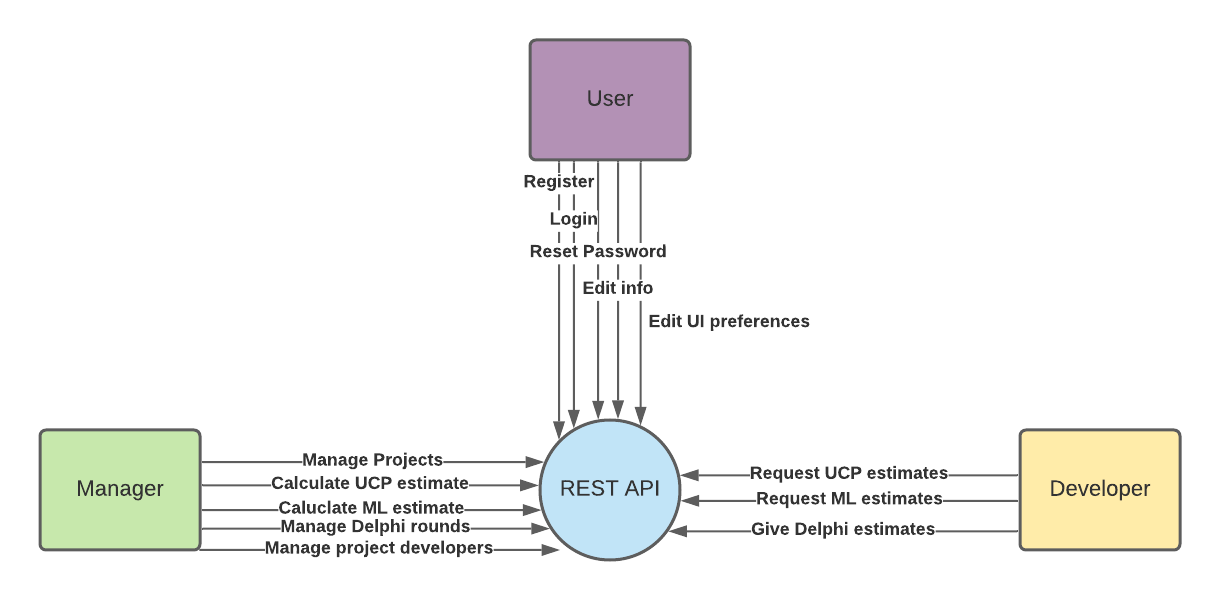
\includegraphics[scale=0.7]{./diagrams/data-flow/df-1.png}
    \label{fig:df-diag-1}
\end{figure}


\subsubsection{Level 2}
\begin{figure}[H]
    \centering
    \caption{Data Flow Diagram 2}
    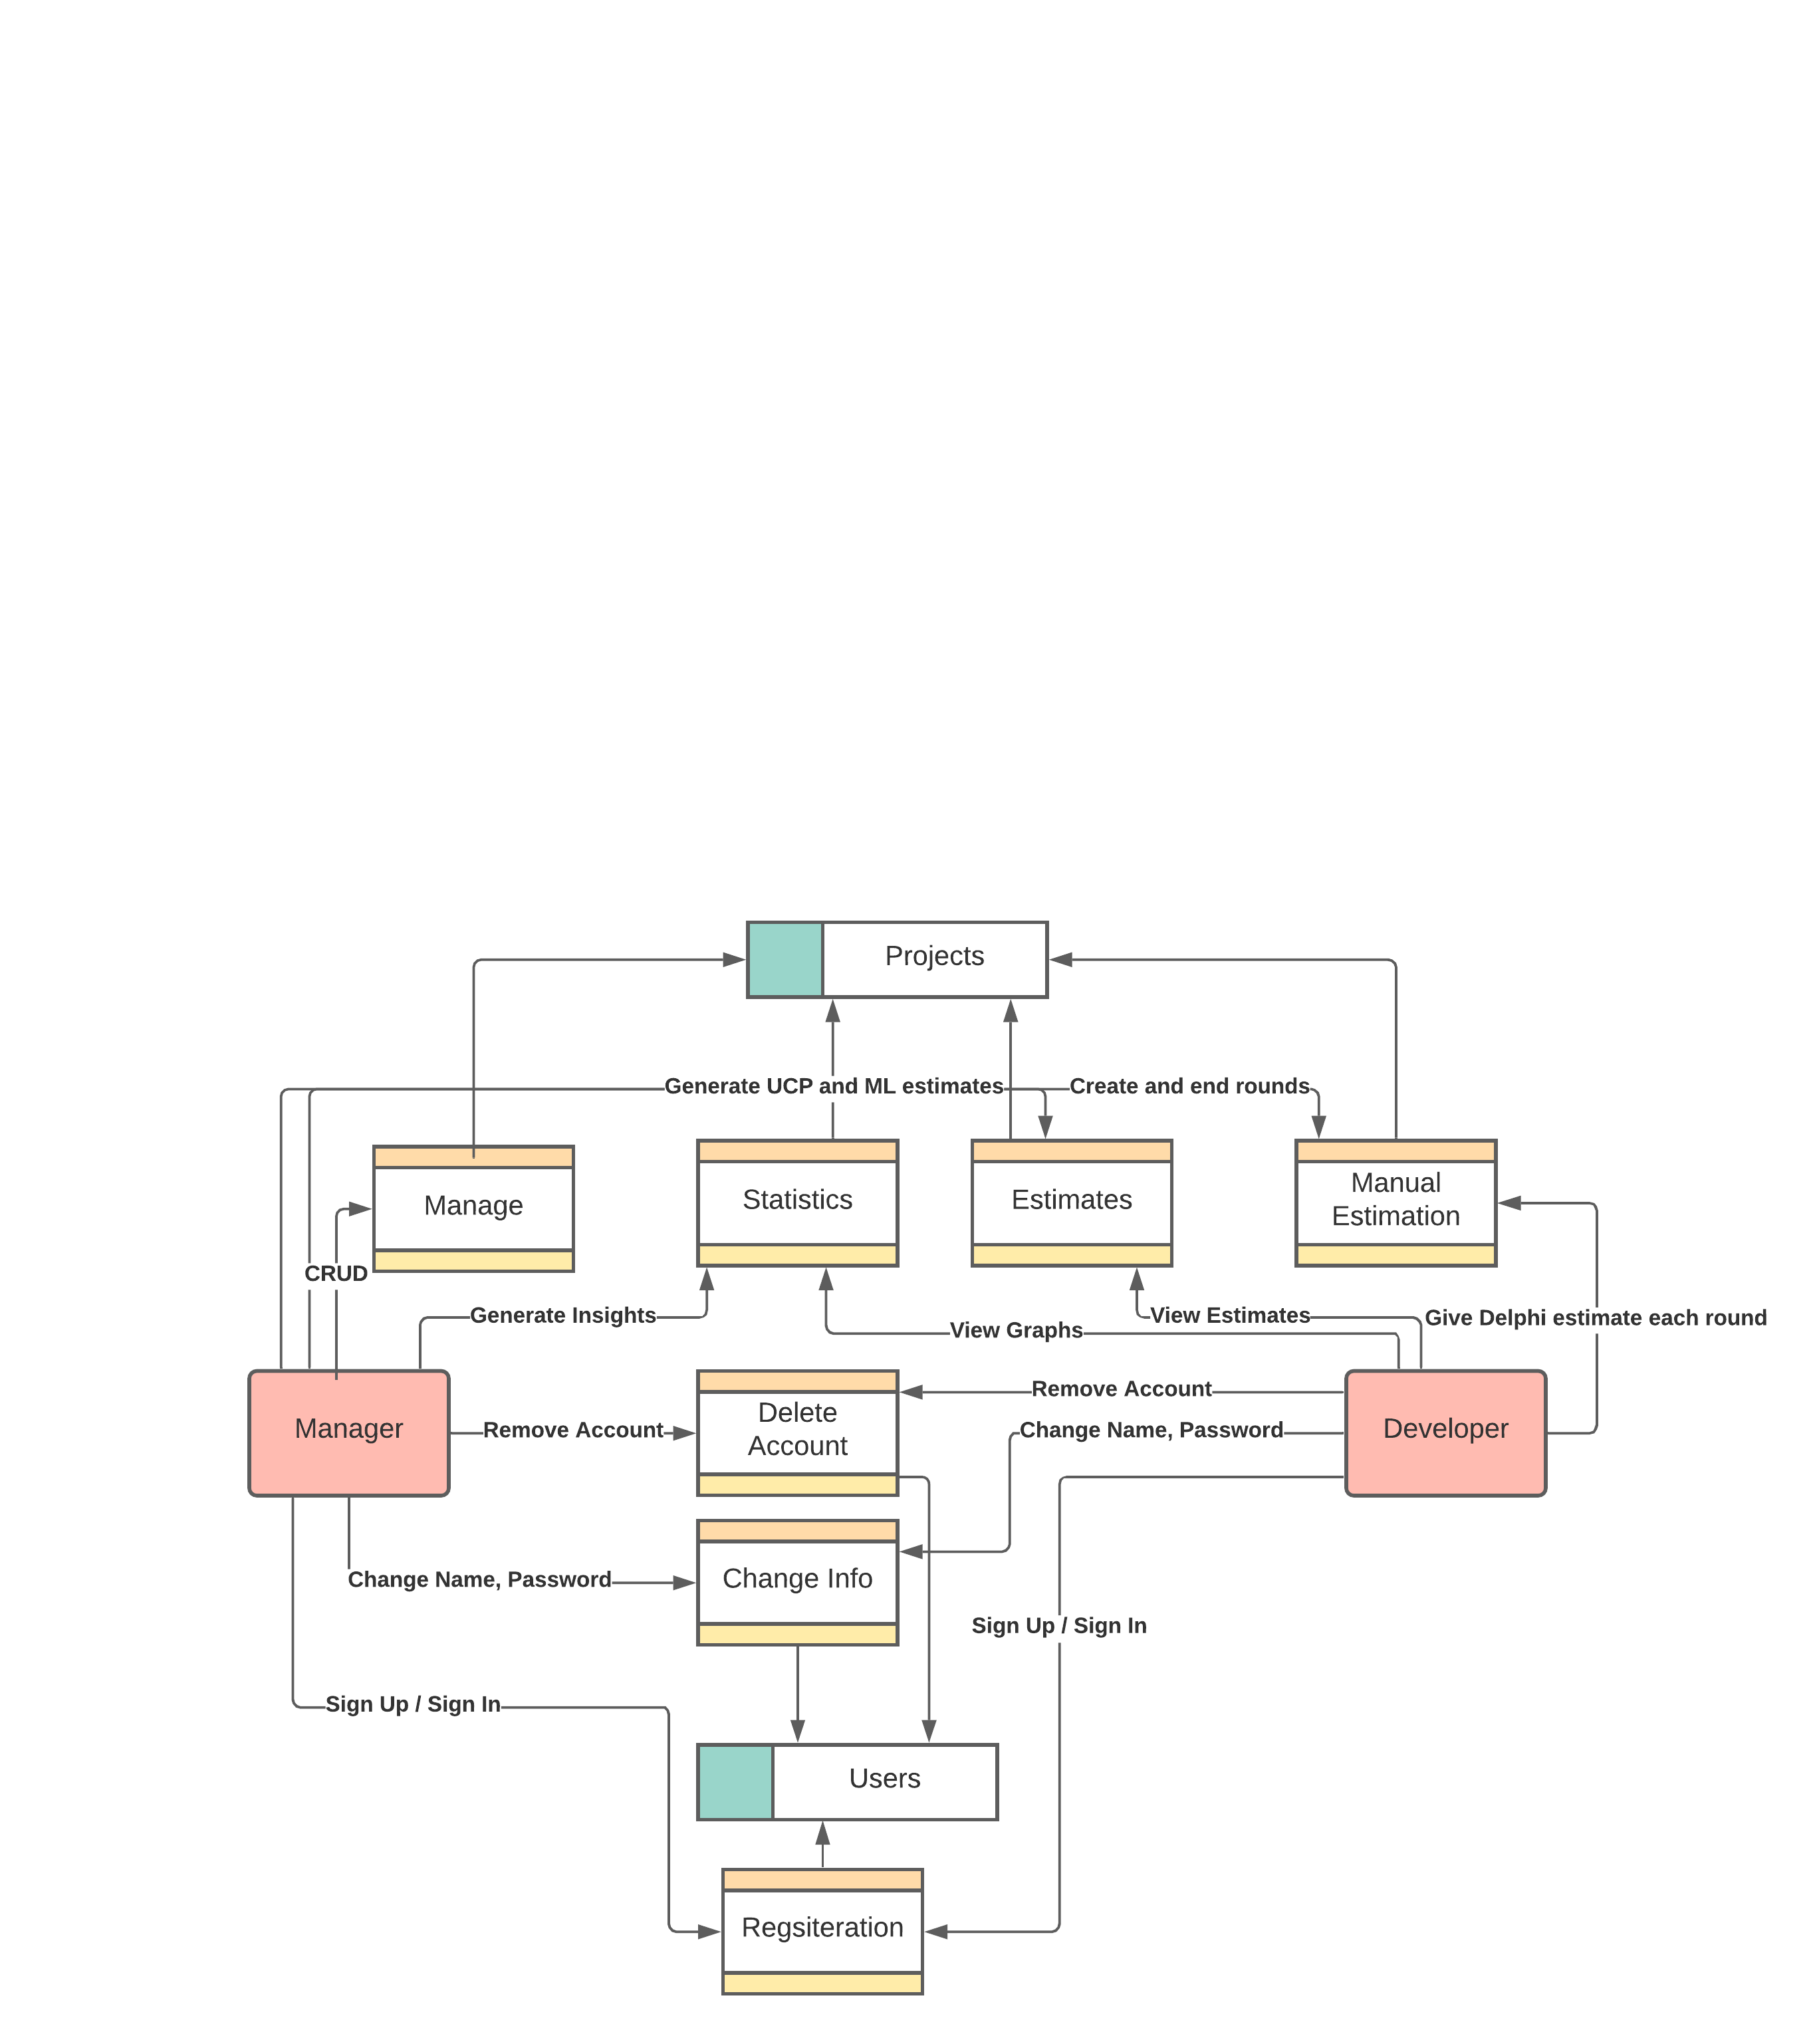
\includegraphics[scale=0.7]{./diagrams/data-flow/df-2.png}
    \label{fig:df-diag-2}
\end{figure}


% Activity Diagram
\subsection{Activity Diagram}

\begin{figure}[H]
    \centering
    \caption{Activity Diagram 1}
    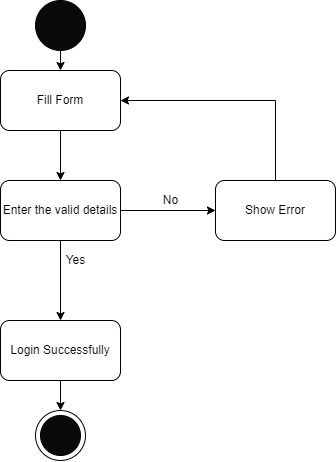
\includegraphics[scale=0.5]{./diagrams/Activity Diagram/ad-01.png}
    \label{fig:act-01}

\end{figure}


\begin{figure}[H]
    \centering
    \caption{Activity Diagram 2}
    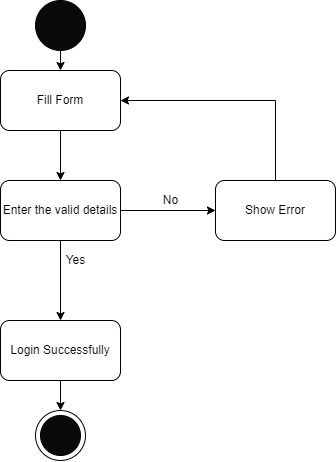
\includegraphics[scale=0.5]{./diagrams/Activity Diagram/ad-02.png}
    \label{fig:act-02}

\end{figure}


\begin{figure}[H]
    \centering
    \caption{Activity Diagram 3}
    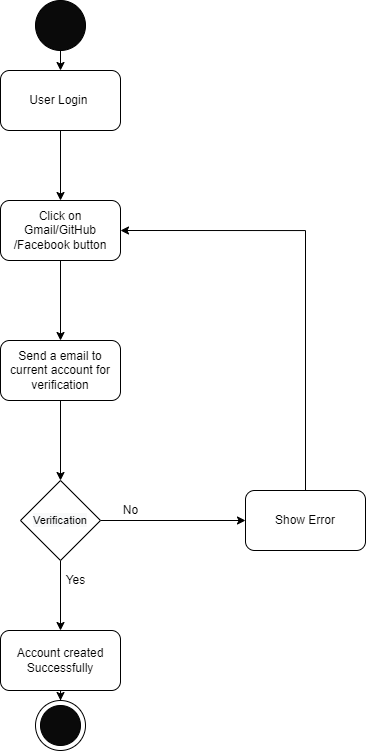
\includegraphics[scale=0.5]{./diagrams/Activity Diagram/ad-03.png}
    \label{fig:act-03}

\end{figure}


\begin{figure}[H]
    \centering
    \caption{Activity Diagram 4}
    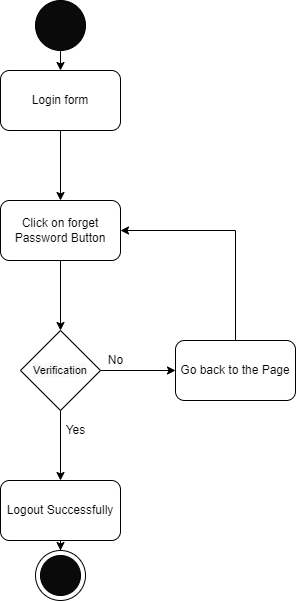
\includegraphics[scale=0.5]{./diagrams/Activity Diagram/ad-04.png}
    \label{fig:act-04}

\end{figure}


\begin{figure}[H]
    \centering
    \caption{Activity Diagram 5}
    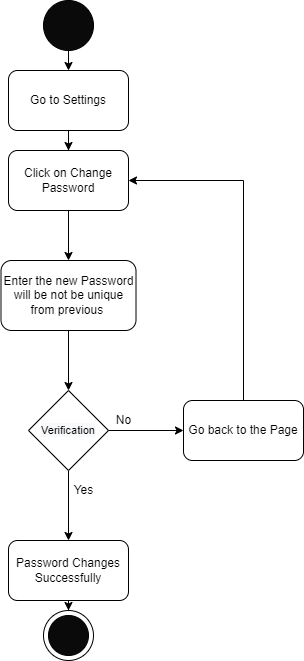
\includegraphics[scale=0.5]{./diagrams/Activity Diagram/ad-05.png}
    \label{fig:act-05}

\end{figure}


\begin{figure}[H]
    \centering
    \caption{Activity Diagram 6}
    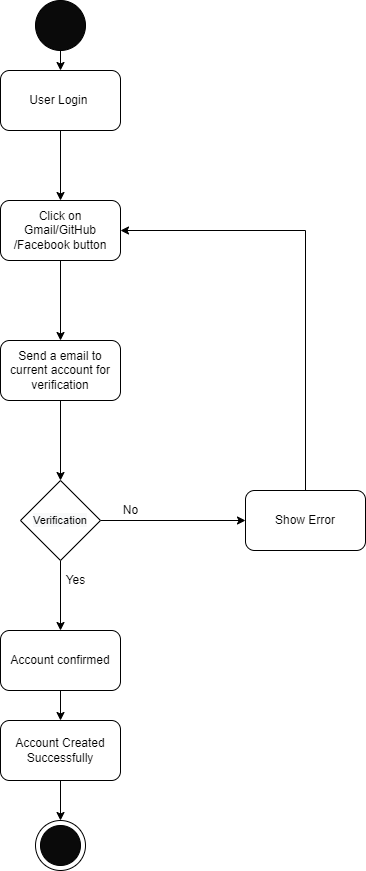
\includegraphics[scale=0.5]{./diagrams/Activity Diagram/ad-06.png}
    \label{fig:act-06}

\end{figure}


\begin{figure}[H]
    \centering
    \caption{Activity Diagram 7}
    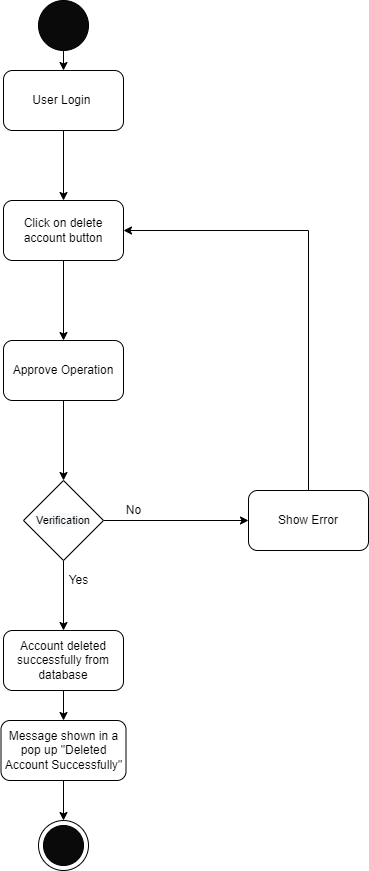
\includegraphics[scale=0.5]{./diagrams/Activity Diagram/ad-07.png}
    \label{fig:act-07}

\end{figure}


\begin{figure}[H]
    \centering
    \caption{Activity Diagram 8}
    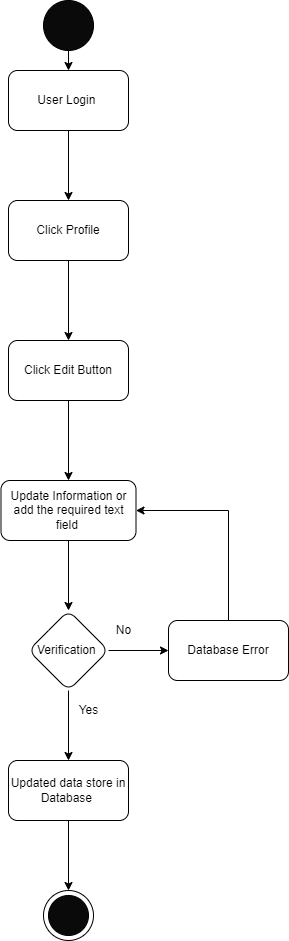
\includegraphics[scale=0.5]{./diagrams/Activity Diagram/ad-08.png}
    \label{fig:act-08}

\end{figure}


\begin{figure}[H]
    \centering
    \caption{Activity Diagram 9}
    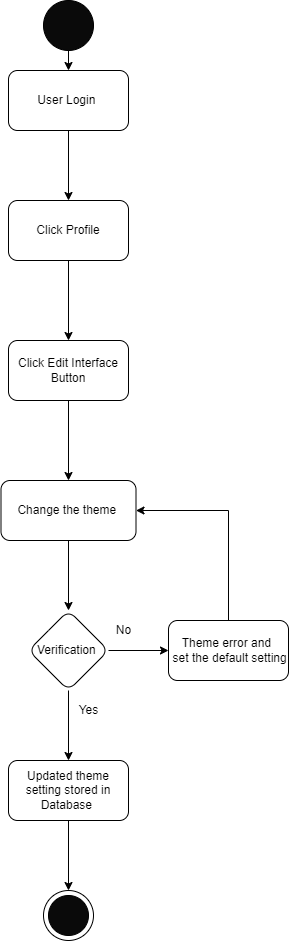
\includegraphics[scale=0.5]{./diagrams/Activity Diagram/ad-09.png}
    \label{fig:act-09}

\end{figure}


\begin{figure}[H]
    \centering
    \caption{Activity Diagram 10}
    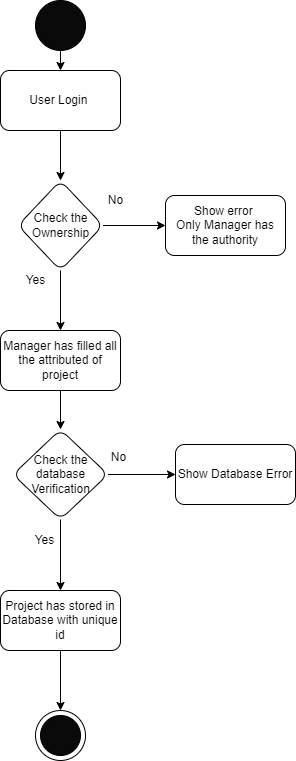
\includegraphics[scale=0.5]{./diagrams/Activity Diagram/ad-10.png}
    \label{fig:act-10}

\end{figure}


\begin{figure}[H]
    \centering
    \caption{Activity Diagram 11}
    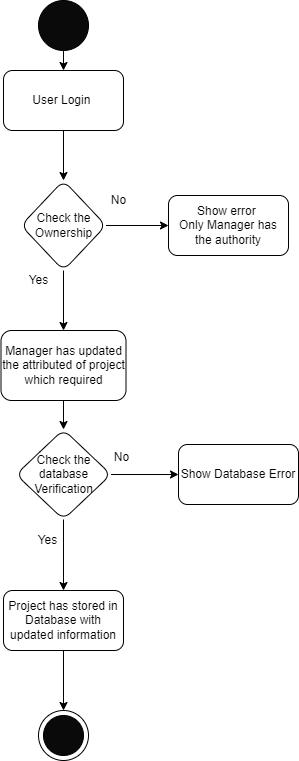
\includegraphics[scale=0.5]{./diagrams/Activity Diagram/ad-11.png}
    \label{fig:act-11}

\end{figure}


\begin{figure}[H]
    \centering
    \caption{Activity Diagram 12}
    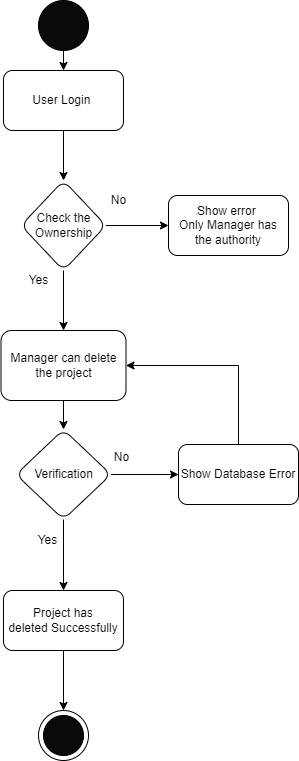
\includegraphics[scale=0.5]{./diagrams/Activity Diagram/ad-12.png}
    \label{fig:act-12}

\end{figure}


\begin{figure}[H]
    \centering
    \caption{Activity Diagram 13}
    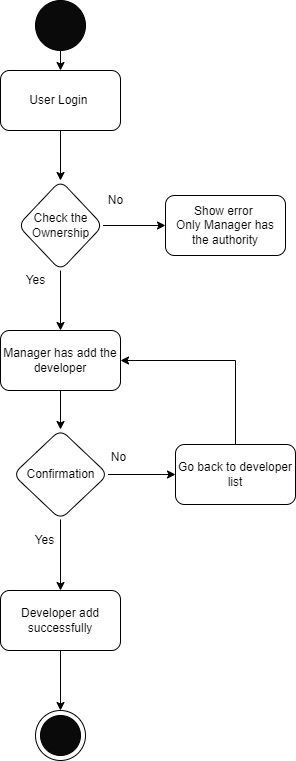
\includegraphics[scale=0.5]{./diagrams/Activity Diagram/ad-13.png}
    \label{fig:act-13}

\end{figure}


\begin{figure}[H]
    \centering
    \caption{Activity Diagram 14}
    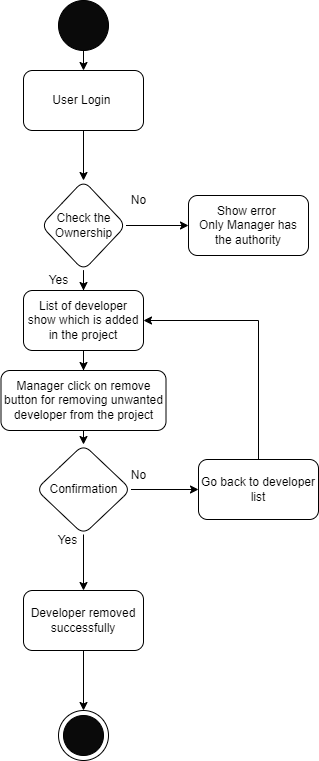
\includegraphics[scale=0.5]{./diagrams/Activity Diagram/ad-14.png}
    \label{fig:act-14}

\end{figure}


\begin{figure}[H]
    \centering
    \caption{Activity Diagram 15}
    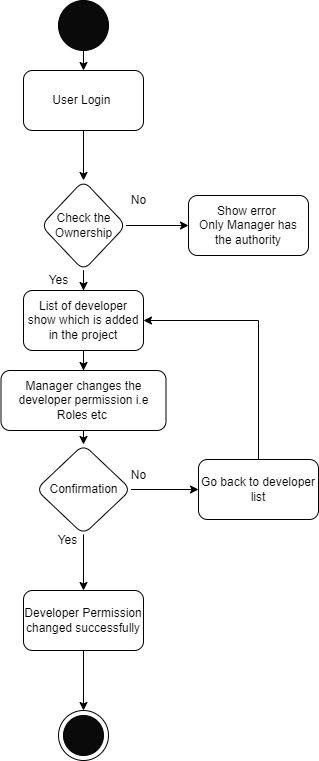
\includegraphics[scale=0.5]{./diagrams/Activity Diagram/ad-15.png}
    \label{fig:act-15}

\end{figure}


\begin{figure}[H]
    \centering
    \caption{Activity Diagram 16}
    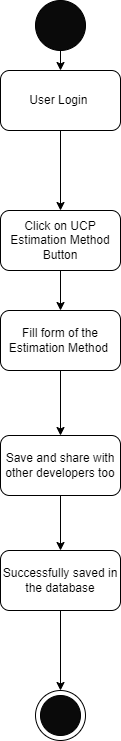
\includegraphics[scale=0.5]{./diagrams/Activity Diagram/ad-16.png}
    \label{fig:act-16}

\end{figure}


\begin{figure}[H]
    \centering
    \caption{Activity Diagram 17}
    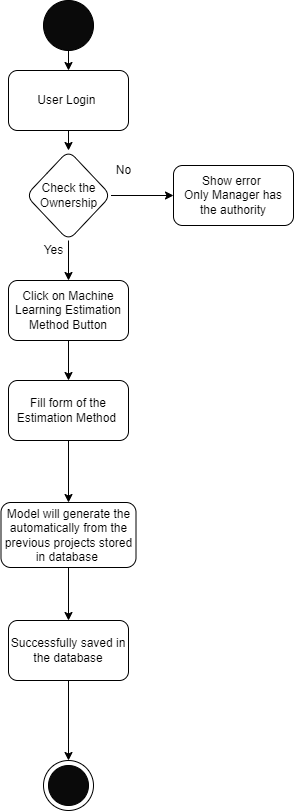
\includegraphics[scale=0.5]{./diagrams/Activity Diagram/ad-17.png}
    \label{fig:act-17}

\end{figure}


\begin{figure}[H]
    \centering
    \caption{Activity Diagram 18}
    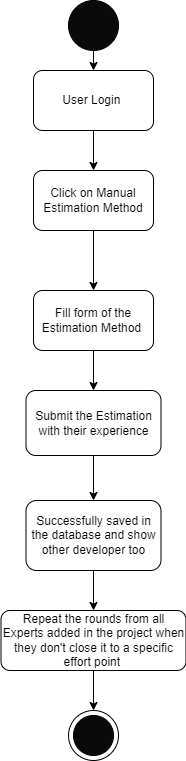
\includegraphics[scale=0.5]{./diagrams/Activity Diagram/ad-18.png}
    \label{fig:act-18}

\end{figure}


\begin{figure}[H]
    \centering
    \caption{Activity Diagram 19}
    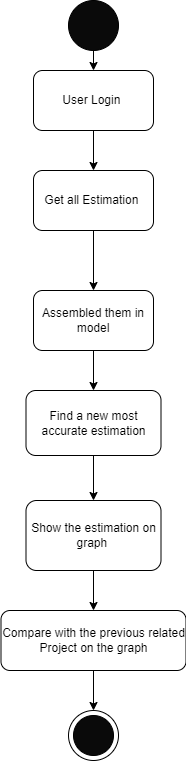
\includegraphics[scale=0.5]{./diagrams/Activity Diagram/ad-19.png}
    \label{fig:act-19}

\end{figure}


\begin{figure}[H]
    \centering
    \caption{Activity Diagram 1}
    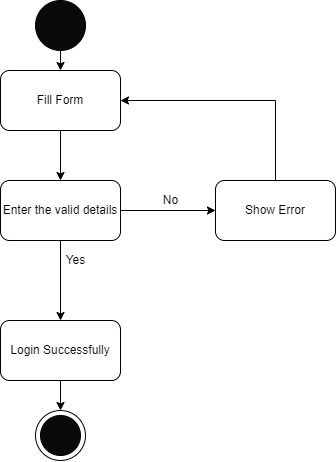
\includegraphics[scale=0.5]{./diagrams/Activity Diagram/ad-01.png}
    \label{fig:act-01}

\end{figure}


\begin{figure}[H]
    \centering
    \caption{Activity Diagram 2}
    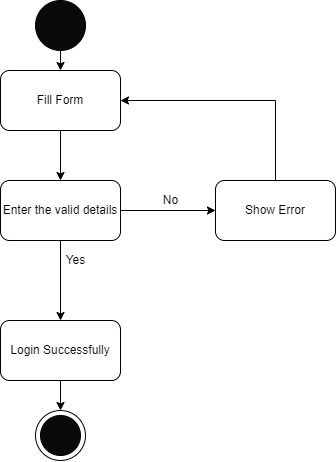
\includegraphics[scale=0.5]{./diagrams/Activity Diagram/ad-02.png}
    \label{fig:act-02}

\end{figure}


\begin{figure}[H]
    \centering
    \caption{Activity Diagram 3}
    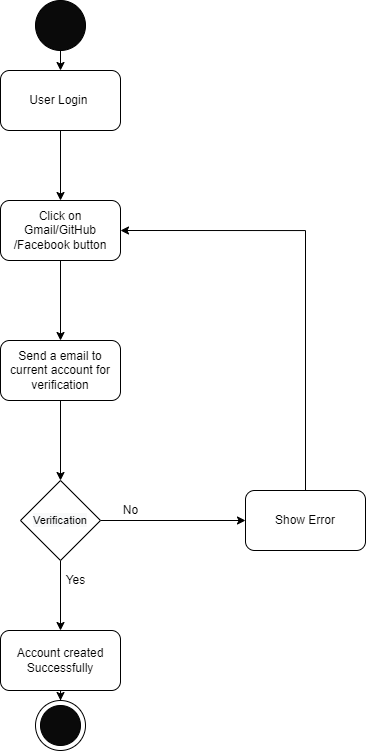
\includegraphics[scale=0.5]{./diagrams/Activity Diagram/ad-03.png}
    \label{fig:act-03}

\end{figure}


\begin{figure}[H]
    \centering
    \caption{Activity Diagram 4}
    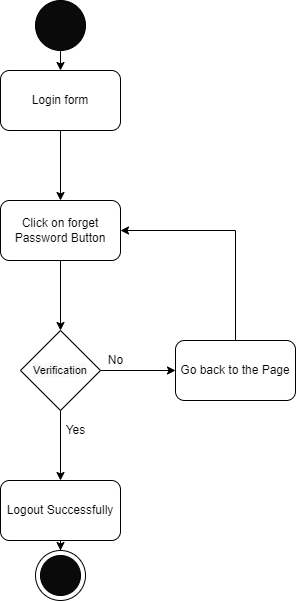
\includegraphics[scale=0.5]{./diagrams/Activity Diagram/ad-04.png}
    \label{fig:act-04}

\end{figure}


\begin{figure}[H]
    \centering
    \caption{Activity Diagram 5}
    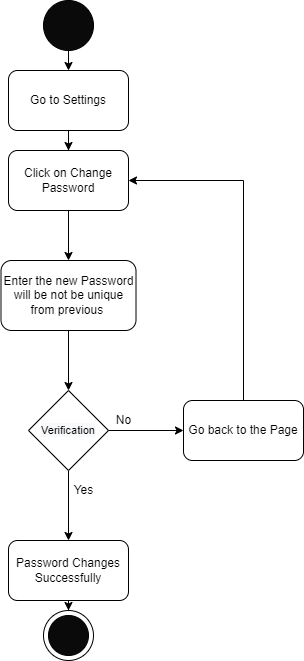
\includegraphics[scale=0.5]{./diagrams/Activity Diagram/ad-05.png}
    \label{fig:act-05}

\end{figure}


\begin{figure}[H]
    \centering
    \caption{Activity Diagram 6}
    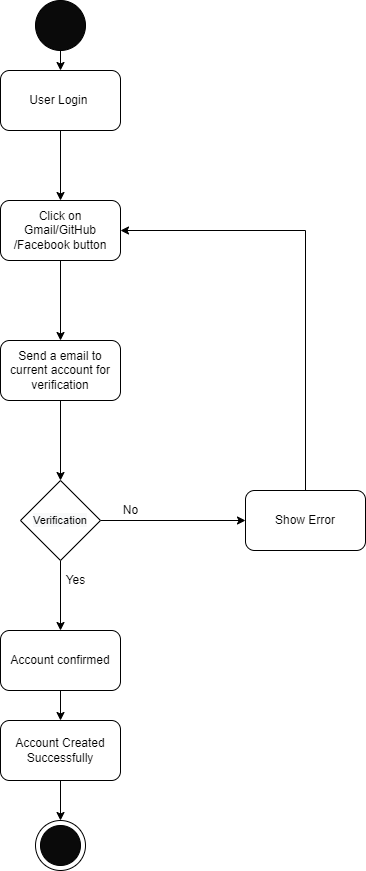
\includegraphics[scale=0.5]{./diagrams/Activity Diagram/ad-06.png}
    \label{fig:act-06}

\end{figure}


\begin{figure}[H]
    \centering
    \caption{Activity Diagram 7}
    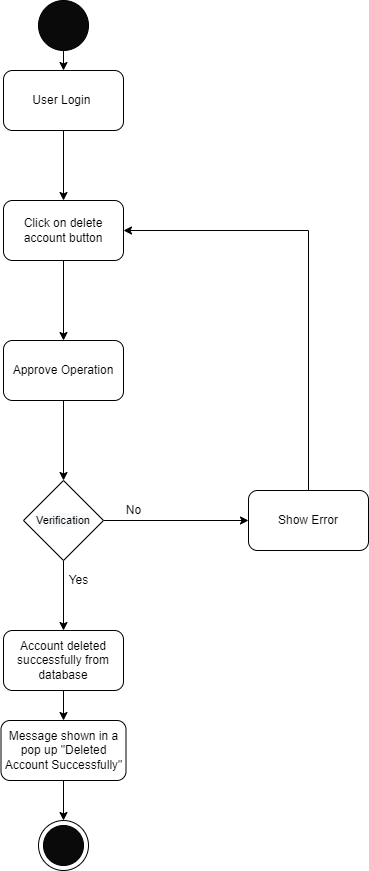
\includegraphics[scale=0.5]{./diagrams/Activity Diagram/ad-07.png}
    \label{fig:act-07}

\end{figure}


\begin{figure}[H]
    \centering
    \caption{Activity Diagram 8}
    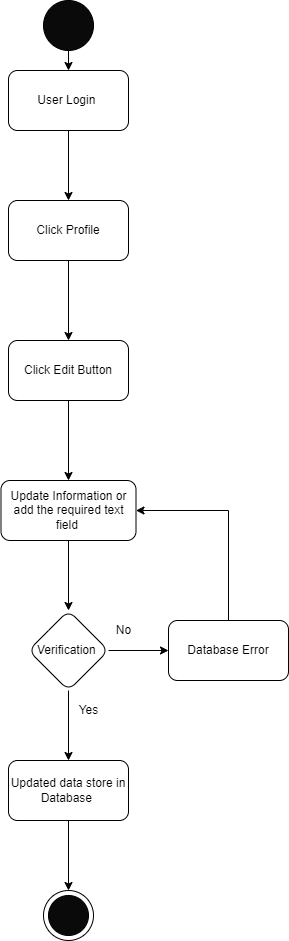
\includegraphics[scale=0.5]{./diagrams/Activity Diagram/ad-08.png}
    \label{fig:act-08}

\end{figure}


\begin{figure}[H]
    \centering
    \caption{Activity Diagram 9}
    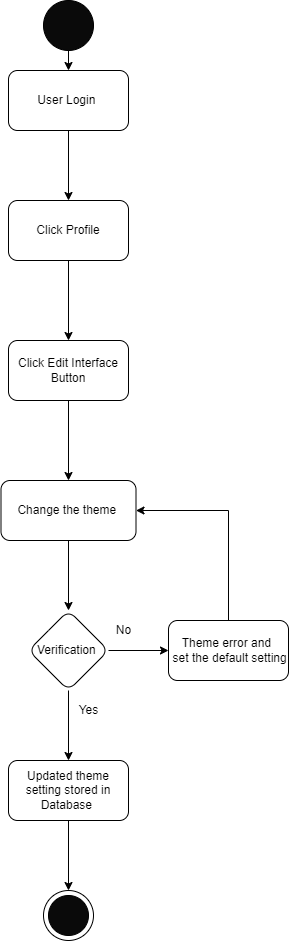
\includegraphics[scale=0.5]{./diagrams/Activity Diagram/ad-09.png}
    \label{fig:act-09}

\end{figure}


\begin{figure}[H]
    \centering
    \caption{Activity Diagram 10}
    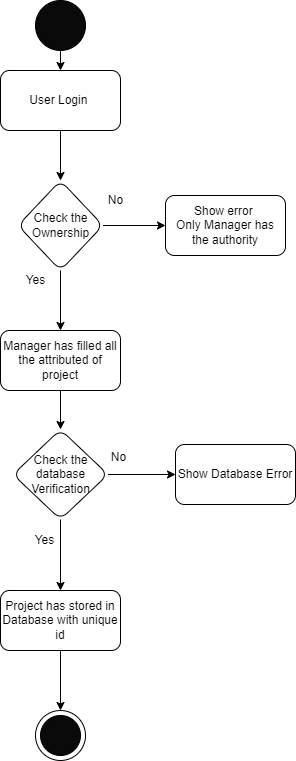
\includegraphics[scale=0.5]{./diagrams/Activity Diagram/ad-10.png}
    \label{fig:act-10}

\end{figure}


\begin{figure}[H]
    \centering
    \caption{Activity Diagram 11}
    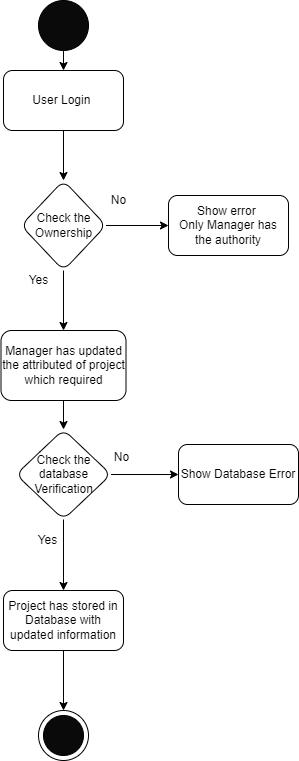
\includegraphics[scale=0.5]{./diagrams/Activity Diagram/ad-11.png}
    \label{fig:act-11}

\end{figure}


\begin{figure}[H]
    \centering
    \caption{Activity Diagram 12}
    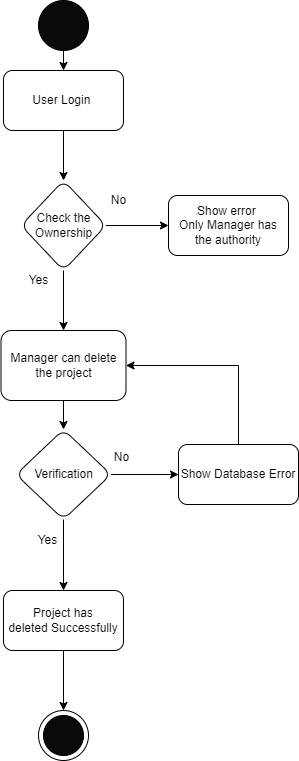
\includegraphics[scale=0.5]{./diagrams/Activity Diagram/ad-12.png}
    \label{fig:act-12}

\end{figure}


\begin{figure}[H]
    \centering
    \caption{Activity Diagram 13}
    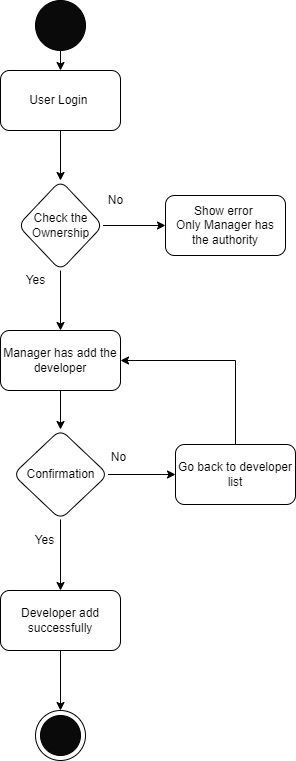
\includegraphics[scale=0.5]{./diagrams/Activity Diagram/ad-13.png}
    \label{fig:act-13}

\end{figure}


\begin{figure}[H]
    \centering
    \caption{Activity Diagram 14}
    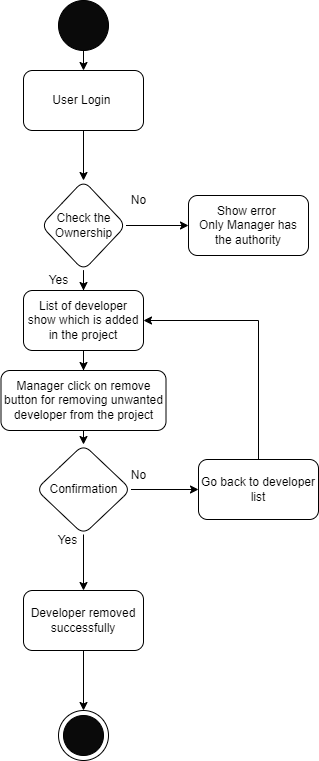
\includegraphics[scale=0.5]{./diagrams/Activity Diagram/ad-14.png}
    \label{fig:act-14}

\end{figure}


\begin{figure}[H]
    \centering
    \caption{Activity Diagram 15}
    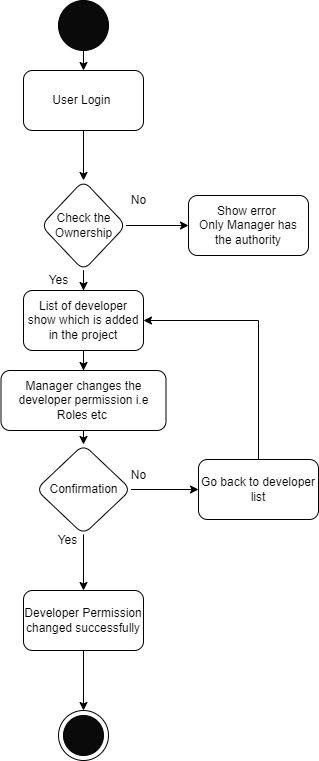
\includegraphics[scale=0.5]{./diagrams/Activity Diagram/ad-15.png}
    \label{fig:act-15}

\end{figure}


\begin{figure}[H]
    \centering
    \caption{Activity Diagram 16}
    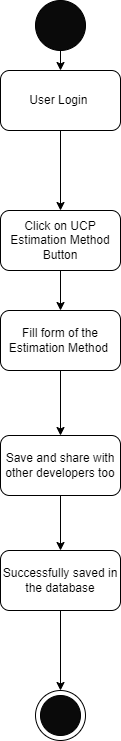
\includegraphics[scale=0.5]{./diagrams/Activity Diagram/ad-16.png}
    \label{fig:act-16}

\end{figure}


\begin{figure}[H]
    \centering
    \caption{Activity Diagram 17}
    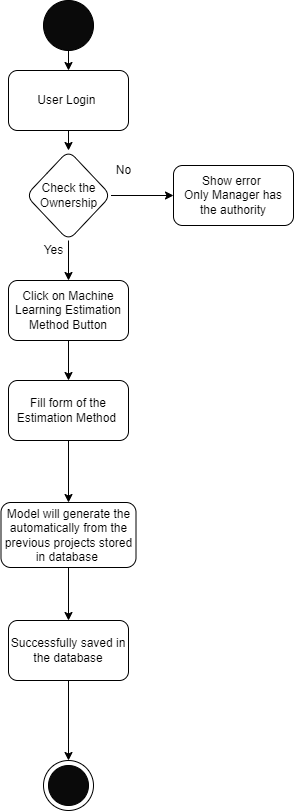
\includegraphics[scale=0.5]{./diagrams/Activity Diagram/ad-17.png}
    \label{fig:act-17}

\end{figure}


\begin{figure}[H]
    \centering
    \caption{Activity Diagram 18}
    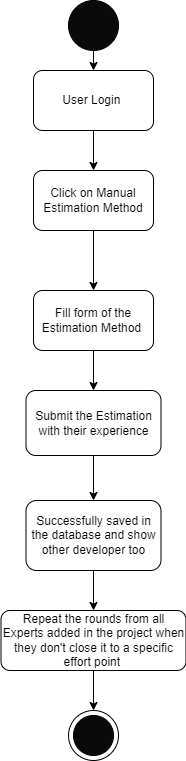
\includegraphics[scale=0.5]{./diagrams/Activity Diagram/ad-18.png}
    \label{fig:act-18}

\end{figure}


\begin{figure}[H]
    \centering
    \caption{Activity Diagram 19}
    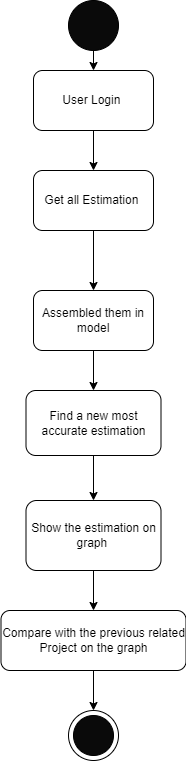
\includegraphics[scale=0.5]{./diagrams/Activity Diagram/ad-19.png}
    \label{fig:act-19}

\end{figure}


\begin{figure}[H]
    \centering
    \caption{Activity Diagram 20}
    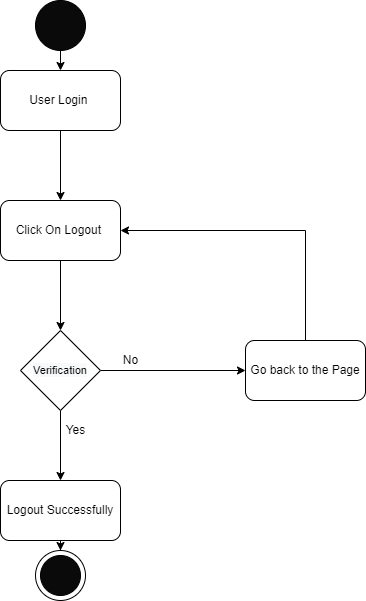
\includegraphics[scale=0.5]{./diagrams/Activity Diagram/ad-20.png}
    \label{fig:act-20}

\end{figure}



% Sequence Diagram
\subsection{Sequence Diagram}

\begin{figure}[H]
    \centering
    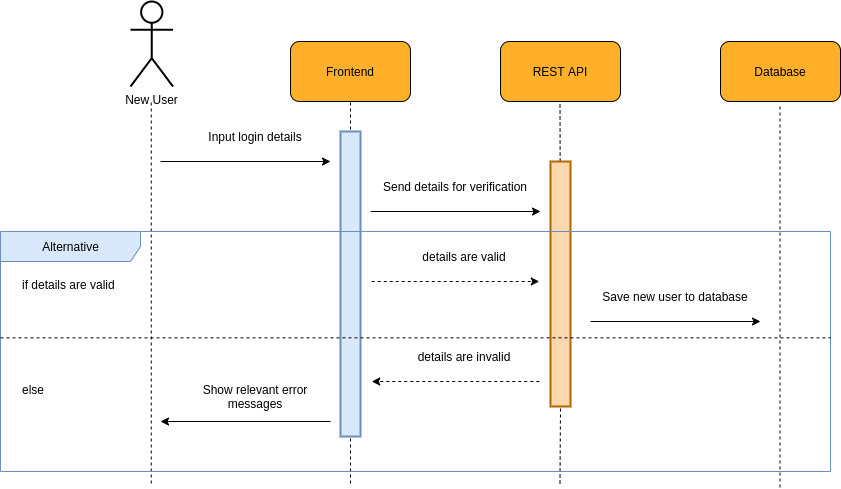
\includegraphics[scale=0.5]{./diagrams/sequence/seq-01.png}
    \caption{Sequence Diagram of UC-1}
    \label{fig:seq-01}
    
\end{figure}


\begin{figure}[H]
    \centering
    \includegraphics[scale=0.5]{./diagrams/sequence/seq-02.png}
    \caption{Sequence Diagram of UC-2}
    \label{fig:seq-02}
    
\end{figure}


\begin{figure}[H]
    \centering
    \includegraphics[scale=0.5]{./diagrams/sequence/seq-03.png}
    \caption{Sequence Diagram of UC-3}
    \label{fig:seq-03}
    
\end{figure}


\begin{figure}[H]
    \centering
    \includegraphics[scale=0.5]{./diagrams/sequence/seq-04.png}
    \caption{Sequence Diagram of UC-4}
    \label{fig:seq-04}
    
\end{figure}


\begin{figure}[H]
    \centering
    \includegraphics[scale=0.5]{./diagrams/sequence/seq-05.png}
    \caption{Sequence Diagram of UC-5}
    \label{fig:seq-05}
    
\end{figure}


\begin{figure}[H]
    \centering
    \includegraphics[scale=0.5]{./diagrams/sequence/seq-06.png}
    \caption{Sequence Diagram of UC-6}
    \label{fig:seq-06}
    
\end{figure}


\begin{figure}[H]
    \centering
    \includegraphics[scale=0.5]{./diagrams/sequence/seq-07.png}
    \caption{Sequence Diagram of UC-7}
    \label{fig:seq-07}
    
\end{figure}


\begin{figure}[H]
    \centering
    \includegraphics[scale=0.5]{./diagrams/sequence/seq-08.png}
    \caption{Sequence Diagram of UC-8}
    \label{fig:seq-08}
    
\end{figure}


\begin{figure}[H]
    \centering
    \includegraphics[scale=0.5]{./diagrams/sequence/seq-09.png}
    \caption{Sequence Diagram of UC-9}
    \label{fig:seq-09}
    
\end{figure}


\begin{figure}[H]
    \centering
    \includegraphics[scale=0.5]{./diagrams/sequence/seq-10.png}
    \caption{Sequence Diagram of UC-10}
    \label{fig:seq-10}
    
\end{figure}


\begin{figure}[H]
    \centering
    \includegraphics[scale=0.5]{./diagrams/sequence/seq-11.png}
    \caption{Sequence Diagram of UC-11}
    \label{fig:seq-11}
    
\end{figure}


\begin{figure}[H]
    \centering
    \includegraphics[scale=0.5]{./diagrams/sequence/seq-12.png}
    \caption{Sequence Diagram of UC-12}
    \label{fig:seq-12}
    
\end{figure}


\begin{figure}[H]
    \centering
    \includegraphics[scale=0.5]{./diagrams/sequence/seq-13.png}
    \caption{Sequence Diagram of UC-13}
    \label{fig:seq-13}
    
\end{figure}


\begin{figure}[H]
    \centering
    \includegraphics[scale=0.5]{./diagrams/sequence/seq-14.png}
    \caption{Sequence Diagram of UC-14}
    \label{fig:seq-14}
    
\end{figure}


\begin{figure}[H]
    \centering
    \includegraphics[scale=0.5]{./diagrams/sequence/seq-15.png}
    \caption{Sequence Diagram of UC-15}
    \label{fig:seq-15}
    
\end{figure}


\begin{figure}[H]
    \centering
    \includegraphics[scale=0.5]{./diagrams/sequence/seq-16.png}
    \caption{Sequence Diagram of UC-16}
    \label{fig:seq-16}
    
\end{figure}


\begin{figure}[H]
    \centering
    \includegraphics[scale=0.5]{./diagrams/sequence/seq-17.png}
    \caption{Sequence Diagram of UC-17}
    \label{fig:seq-17}
    
\end{figure}


\begin{figure}[H]
    \centering
    \includegraphics[scale=0.5]{./diagrams/sequence/seq-18.png}
    \caption{Sequence Diagram of UC-18}
    \label{fig:seq-18}
    
\end{figure}


\begin{figure}[H]
    \centering
    \includegraphics[scale=0.5]{./diagrams/sequence/seq-19.png}
    \caption{Sequence Diagram of UC-19}
    \label{fig:seq-19}
    
\end{figure}



% Collaboration Diagram
% \subsection{Collaboration Diagram}


\begin{figure}[H]
    \centering
    \includegraphics[scale=0.5]{./diagrams/collaboration/cd-1.png}
    \caption{Collaboration diagram of UC-1}
    \label{fig:cd-01}
    
\end{figure}


\begin{figure}[H]
    \centering
    \includegraphics[scale=0.5]{./diagrams/collaboration/cd-2.png}
    \caption{Collaboration diagram of UC-2}
    \label{fig:cd-02}
    
\end{figure}


\begin{figure}[H]
    \centering
    \includegraphics[scale=0.5]{./diagrams/collaboration/cd-3.png}
    \caption{Collaboration diagram of UC-3}
    \label{fig:cd-03}
    
\end{figure}


\begin{figure}[H]
    \centering
    \includegraphics[scale=0.5]{./diagrams/collaboration/cd-4.png}
    \caption{Collaboration diagram of UC-4}
    \label{fig:cd-04}
    
\end{figure}


\begin{figure}[H]
    \centering
    \includegraphics[scale=0.5]{./diagrams/collaboration/cd-5.png}
    \caption{Collaboration diagram of UC-5}
    \label{fig:cd-05}
    
\end{figure}


\begin{figure}[H]
    \centering
    \includegraphics[scale=0.5]{./diagrams/collaboration/cd-6.png}
    \caption{Collaboration diagram of UC-6}
    \label{fig:cd-06}
    
\end{figure}


\begin{figure}[H]
    \centering
    \includegraphics[scale=0.5]{./diagrams/collaboration/cd-7.png}
    \caption{Collaboration diagram of UC-7}
    \label{fig:cd-07}
    
\end{figure}


\begin{figure}[H]
    \centering
    \includegraphics[scale=0.5]{./diagrams/collaboration/cd-8.png}
    \caption{Collaboration diagram of UC-8}
    \label{fig:cd-08}
    
\end{figure}


\begin{figure}[H]
    \centering
    \includegraphics[scale=0.5]{./diagrams/collaboration/cd-9.png}
    \caption{Collaboration diagram of UC-9}
    \label{fig:cd-09}
    
\end{figure}


\begin{figure}[H]
    \centering
    \includegraphics[scale=0.5]{./diagrams/collaboration/cd-10.png}
    \caption{Collaboration diagram of UC-10}
    \label{fig:cd-10}
    
\end{figure}


\begin{figure}[H]
    \centering
    \includegraphics[scale=0.5]{./diagrams/collaboration/cd-11.png}
    \caption{Collaboration diagram of UC-11}
    \label{fig:cd-11}
    
\end{figure}


\begin{figure}[H]
    \centering
    \includegraphics[scale=0.5]{./diagrams/collaboration/cd-12.png}
    \caption{Collaboration diagram of UC-12}
    \label{fig:cd-12}
    
\end{figure}


\begin{figure}[H]
    \centering
    \includegraphics[scale=0.5]{./diagrams/collaboration/cd-13.png}
    \caption{Collaboration diagram of UC-13}
    \label{fig:cd-13}
    
\end{figure}


\begin{figure}[H]
    \centering
    \includegraphics[scale=0.5]{./diagrams/collaboration/cd-14.png}
    \caption{Collaboration diagram of UC-14}
    \label{fig:cd-14}
    
\end{figure}


\begin{figure}[H]
    \centering
    \includegraphics[scale=0.5]{./diagrams/collaboration/cd-15.png}
    \caption{Collaboration diagram of UC-15}
    \label{fig:cd-15}
    
\end{figure}


\begin{figure}[H]
    \centering
    \includegraphics[scale=0.5]{./diagrams/collaboration/cd-16.png}
    \caption{Collaboration diagram of UC-16}
    \label{fig:cd-16}
    
\end{figure}


\begin{figure}[H]
    \centering
    \includegraphics[scale=0.5]{./diagrams/collaboration/cd-17.png}
    \caption{Collaboration diagram of UC-17}
    \label{fig:cd-17}
    
\end{figure}


\begin{figure}[H]
    \centering
    \includegraphics[scale=0.5]{./diagrams/collaboration/cd-18.png}
    \caption{Collaboration diagram of UC-18}
    \label{fig:cd-18}
    
\end{figure}


\begin{figure}[H]
    \centering
    \includegraphics[scale=0.5]{./diagrams/collaboration/cd-19.png}
    \caption{Collaboration diagram of UC-19}
    \label{fig:cd-19}
    
\end{figure}



% State Transition Diagram
\subsection{State Transition Diagram}
\begin{figure}[H]
    \centering
    \includegraphics[scale=0.7]{./diagrams/state-transition.png}
    \caption{State Transition Diagram}
    \label{fig:state-transition}
\end{figure}


% Component Diagram
\subsection{Component Diagram}
\begin{figure}[H]
    \centering
    \includegraphics[scale=0.6]{./diagrams/component-diagram.png}
    \caption{Component Diagram}
    \label{fig:component}
\end{figure}

% Deployment Diagram
\subsection{Deployment Diagram}
\begin{figure}[H]
    \centering
    \includegraphics[scale=0.6]{./diagrams/deployment-diagram.png}
    \caption{Deployment Diagram}
    \label{fig:deployment}
\end{figure}
